\documentclass[11pt,letterpaper]{article}

\usepackage[T1]{fontenc}
\usepackage{amsmath,amssymb}
\usepackage{booktabs}
\usepackage[margin=2.5cm]{geometry}
\usepackage{graphicx}
\usepackage{tabularx}
\usepackage{array}
\usepackage{url}
\usepackage{subcaption}
\usepackage{float}
\usepackage{fancyhdr}
\usepackage[hidelinks]{hyperref}

\newcolumntype{Y}{>{\raggedright\arraybackslash}X}

\setlength{\parindent}{0pt}
\setlength{\parskip}{0.55em}
\setlength{\floatsep}{1.0em}
\setlength{\textfloatsep}{1.1em}
\setlength{\intextsep}{1.0em}
\setlength{\emergencystretch}{2em}
\renewcommand{\arraystretch}{1.14}
\setcounter{tocdepth}{2}

\pagestyle{fancy}
\fancyhf{}
\rhead{\small Workshop No. 5 -- Generative Adversarial Networks}
\lhead{\small Machine Learning (2026-III) -- Gr. 1}
\rfoot{\small Page \thepage}

\begin{document}

\hypersetup{pageanchor=false}
\begin{titlepage}
\centering
\vspace*{1.0cm}
{\Large\bfseries Universidad Distrital Francisco Jos\'e de Caldas\par}
\vspace{0.55cm}
{\large Faculty of Engineering\par}
{\large Computer Engineering Program\par}

\vfill
{\Large\bfseries Workshop No. 5 -- Generative Adversarial Networks\par}
\vspace{0.8cm}
{\LARGE\bfseries Adversarial Synthesis, Manifold Evaluation, and\par}
\vspace{0.25cm}
{\LARGE\bfseries Data Augmentation for Tabular Real Estate Valuation\par}

\vfill
{\large\bfseries Group 1 Authors\par}
\vspace{0.5cm}
{\large Miguel Alejandro Ch\'avez Porras -- 20212020033\par}
{\large Luisa Fernanda Guerrero Ordo\~nez -- 20212020099\par}
{\large Dilan Stive Arboleda Zambrano -- 20212020105\par}

\vfill
{\large Machine Learning -- Semester 2026-III\par}
{\large Professor: Eng. Carlos Andr\'es Sierra, M.Sc.\par}
{\large Bogot\'a, Colombia\par}
\vspace{0.5cm}
{\large November 15, 2026\par}
\end{titlepage}

\hypersetup{pageanchor=true}
\pagenumbering{roman}
\tableofcontents
\clearpage
\pagenumbering{arabic}

\begin{abstract}
This report investigates adversarial generative modeling on the benchmark Ames Housing dataset ($N = 2,930$ residential records, 82 raw attributes), establishing an end-to-end framework for synthetic tabular generation, distribution auditing, and downstream data augmentation. Using a strictly leak-free preprocessing pipeline fitted exclusively on the 2,050-property training partition, we construct and benchmark two generative adversarial paradigms: a Vanilla Generative Adversarial Network (Vanilla GAN) utilizing a minimax Jensen-Shannon objective with one-sided label smoothing, and a Wasserstein GAN with 1-Lipschitz Gradient Penalty (WGAN-GP). Quantitative evaluation reveals that WGAN-GP fundamentally outperforms Vanilla GAN across distribution-matching criteria, achieving a Fr\'echet Distance of 0.4719 (versus 0.8582 for Vanilla GAN), a 27.8\% reduction in correlation matrix Frobenius error (3.1115 vs. 4.3136), and superior coverage of the real data manifold without mode collapse. In a controlled downstream data augmentation experiment, retraining the Workshop 2 Multilayer Perceptron (\texttt{HousingMLP}) on augmented synthetic datasets ($N = 4,048$) demonstrates that WGAN-GP data acts as an effective variance regularizer, reducing test Root Mean Squared Error from \$41,283.36 to \$35,777.83 and lifting $R^2$ from 0.7782 to 0.8334 on the untouched 440-property test split. All code, checkpoints, logs, and artifacts are systematically organized and fully reproducible.
\end{abstract}

\noindent\textbf{Keywords:} Generative Adversarial Networks, WGAN-GP, Tabular Synthesis, Fr\'echet Distance, Mode Collapse, Data Augmentation, Ames Housing.

\section{Introduction and Domain Motivation}
Generative Adversarial Networks (GANs), introduced by Goodfellow et al. (2014) \cite{goodfellow2014}, frame generative learning as a zero-sum game between a Generator network $G$ and an adversarial Discriminator $D$. While GANs were originally developed for continuous image domains \cite{radford2015}, generative modeling for structured tabular data addresses critical operational challenges in modern data science: data scarcity in extreme value regimes, privacy-preserving synthetic dataset sharing, and empirical training augmentation \cite{xu2019}.

In real estate valuation, transactions are constrained by regional zoning laws, physical building codes, and macroeconomic market cycles. Certain property tiers---such as bespoke luxury estates, historic homes, or specialized architectural configurations---are inherently scarce in observational registries like the Ames Assessor database \cite{decock2011}. Traditional synthetic sampling techniques (e.g., SMOTE or Gaussian jittering) introduce linear interpolations that ignore structural domain constraints, generating unfeasible feature combinations (such as full masonry veneer on frame-less barns, or negative basement square footage). A deep generative model capable of capturing complex non-linear feature interactions can potentially explore under-sampled regions of the housing manifold and regularize downstream predictors.

This workshop addresses two central research questions:
\begin{enumerate}
    \item \textit{Can an adversarially trained generator synthesize realistic, multi-attribute tabular vectors that accurately replicate the joint distribution and correlation structure of residential real estate?}
    \item \textit{How does synthetic data augmentation impact downstream neural network performance when predicting market valuation on unseen test properties?}
\end{enumerate}

To answer these questions, we implement and contrast a Vanilla GAN against a Wasserstein GAN with Gradient Penalty (WGAN-GP), diagnose adversarial failure modes, evaluate distribution fidelity via quantitative metrics, and benchmark downstream regression performance on the frozen Workshop 2 test split.

\section{Theoretical Framework}

\subsection{Vanilla Generative Adversarial Networks}
The original formulation by Goodfellow et al. (2014) \cite{goodfellow2014} establishes the two-player minimax objective:
\begin{equation}
\min_G \max_D V(D, G) = \mathbb{E}_{x \sim p_{\text{data}}(x)}[\log D(x)] + \mathbb{E}_{z \sim p_z(z)}[\log(1 - D(G(z)))],
\end{equation}
where $z \sim \mathcal{N}(0, I)$ represents a low-dimensional latent noise prior, $G(z)$ is the synthesized sample, and $D(x) \in [0, 1]$ represents the probability that $x$ originates from the empirical data distribution rather than the generator.

When the discriminator is trained to optimality for a fixed generator, $D^*_G(x) = \frac{p_{\text{data}}(x)}{p_{\text{data}}(x) + p_g(x)}$. Substituting this into the minimax objective demonstrates that minimizing $V(D^*_G, G)$ is equivalent to minimizing the Jensen-Shannon Divergence (JSD):
\begin{equation}
V(D^*_G, G) = 2 \cdot D_{\text{JS}}(p_{\text{data}} \parallel p_g) - 2 \log 2.
\end{equation}

\noindent\textbf{Theoretical Limitations and Failure Modes:}
\begin{itemize}
    \item \textit{Vanishing Gradients:} If the support of $p_{\text{data}}$ and $p_g$ lie on lower-dimensional manifolds that do not intersect or have measure-zero intersection, the JSD attains its maximum constant value of $\log 2$. Consequently, the optimal discriminator achieves 100\% classification confidence ($D(x) \approx 1, D(G(z)) \approx 0$), causing the gradient $\nabla_z \log(1 - D(G(z)))$ to vanish entirely \cite{arjovsky2017towards}.
    \item \textit{Mode Collapse:} When the generator discovers a small cluster of samples that easily fools the current discriminator, it concentrates its entire probability mass on that limited subset, failing to capture the full diversity of the underlying data distribution.
\end{itemize}

\subsection{Wasserstein GAN with Gradient Penalty (WGAN-GP)}
To resolve the discontinuities and vanishing gradients inherent in JSD, Arjovsky et al. (2017) \cite{arjovsky2017wgan} proposed replacing divergence metrics with the Earth Mover's (Wasserstein-1) Distance:
\begin{equation}
W(p_{\text{data}}, p_g) = \inf_{\gamma \in \Pi(p_{\text{data}}, p_g)} \mathbb{E}_{(x, y) \sim \gamma}[\|x - y\|],
\end{equation}
which represents the minimal transportation cost required to morph distribution $p_g$ into $p_{\text{data}}$. Via the Kantorovich-Rubinstein duality theorem, the objective is reformulated as:
\begin{equation}
\max_{D \in \mathcal{D}_L} \mathbb{E}_{x \sim p_{\text{data}}}[D(x)] - \mathbb{E}_{\tilde{x} \sim p_g}[D(\tilde{x})],
\end{equation}
where $\mathcal{D}_L$ is the set of 1-Lipschitz continuous functions ($\|D(x_1) - D(x_2)\| \le \|x_1 - x_2\|$).

While original WGAN enforced 1-Lipschitz continuity via weight clipping ($\mathcal{W} \in [-c, c]$), Gulrajani et al. (2017) \cite{gulrajani2017} proved that weight clipping biases the critic toward pathological extremal surfaces. They introduced the 1-Lipschitz Gradient Penalty:
\begin{equation}
L_{\text{critic}} = \mathbb{E}_{\tilde{x} \sim p_g}[D(\tilde{x})] - \mathbb{E}_{x \sim p_{\text{data}}}[D(x)] + \lambda \mathbb{E}_{\hat{x} \sim p_{\hat{x}}}\left[\left(\|\nabla_{\hat{x}} D(\hat{x})\|_2 - 1\right)^2\right],
\end{equation}
where samples $\hat{x} = \epsilon x + (1 - \epsilon)\tilde{x}$ with $\epsilon \sim \mathcal{U}[0, 1]$ are interpolated along straight lines connecting real and synthetic points, and $\lambda = 10$. Crucially, the critic must utilize \texttt{LayerNorm} rather than \texttt{BatchNorm}, since batch normalization introduces cross-sample dependencies that violate the pointwise gradient penalty objective \cite{gulrajani2017}.

\section{System Architecture and Experimental Methodology}

\subsection{Tabular Ingestion and Normalization Strategy}
We ingest the Ames Housing dataset through the unified preprocessing pipeline developed in Workshop 1. Following De Cock's outlier removal on the training partition ($N_{\text{train}} = 2,048$), ordinal ratings are monotonically mapped, missing categorical indicators are treated as explicit absence levels (\texttt{'None'}), and nominal attributes are one-hot encoded, yielding 260 engineered explanatory features.

To enable full joint synthesis of both housing attributes and market price, we concatenate the standardized log-transformed target:
\begin{equation}
\mathbf{x} = \left[\mathbf{X}_{\text{features}}, \log(1 + \text{SalePrice})\right] \in \mathbb{R}^{261}.
\end{equation}
Because the Generator utilizes \texttt{Tanh} activation in its final layer, all 261 continuous and encoded dimensions are scaled into the interval $[-1.0, 1.0]$ using a Min-Max standardizer fitted strictly on the training partition:
\begin{equation}
\tilde{\mathbf{x}} = 2 \cdot \frac{\mathbf{x} - \mathbf{x}_{\min}}{\mathbf{x}_{\max} - \mathbf{x}_{\min}} - 1.0.
\end{equation}

\subsection{Network Topologies}
Table~\ref{tab:architectures} specifies the neural architectures for the Generator, Vanilla Discriminator, and WGAN-GP Critic.

\begin{table}[H]
\centering
\small
\caption{Detailed Layer Topologies for Tabular GAN Architectures}
\label{tab:architectures}
\begin{tabular}{llll}
\toprule
\textbf{Component} & \textbf{Layer Progression} & \textbf{Normalization \& Dropout} & \textbf{Activations} \\
\midrule
\textbf{Generator $G$} & $\text{FC}(64 \to 128)$ & \texttt{BatchNorm1d}(128) & \texttt{LeakyReLU}(0.2) \\
                       & $\text{FC}(128 \to 256)$ & \texttt{BatchNorm1d}(256) & \texttt{LeakyReLU}(0.2) \\
                       & $\text{FC}(256 \to 256)$ & \texttt{BatchNorm1d}(256) & \texttt{LeakyReLU}(0.2) \\
                       & $\text{FC}(256 \to 261)$ & None & \texttt{Tanh} \\
\midrule
\textbf{Discriminator $D$} & $\text{FC}(261 \to 256)$ & None, \texttt{Dropout}(0.25) & \texttt{LeakyReLU}(0.2) \\
(Vanilla GAN)              & $\text{FC}(256 \to 128)$ & None, \texttt{Dropout}(0.25) & \texttt{LeakyReLU}(0.2) \\
                           & $\text{FC}(128 \to 64)$  & None, \texttt{Dropout}(0.25) & \texttt{LeakyReLU}(0.2) \\
                           & $\text{FC}(64 \to 1)$    & None & \texttt{Sigmoid} \\
\midrule
\textbf{Critic $D$}        & $\text{FC}(261 \to 256)$ & \texttt{LayerNorm}(256) & \texttt{LeakyReLU}(0.2) \\
(WGAN-GP)                  & $\text{FC}(256 \to 128)$ & \texttt{LayerNorm}(128) & \texttt{LeakyReLU}(0.2) \\
                           & $\text{FC}(128 \to 64)$  & \texttt{LayerNorm}(64)  & \texttt{LeakyReLU}(0.2) \\
                           & $\text{FC}(64 \to 1)$    & None & None (Linear) \\
\bottomrule
\end{tabular}
\end{table}

\subsection{Training Protocols}
\begin{itemize}
    \item \textbf{Vanilla GAN Setup:} Batch size $B = 64$, Adam optimizer with learning rate $\eta = 2 \times 10^{-4}$ and momentum $\beta_1 = 0.5, \beta_2 = 0.999$. One-sided label smoothing is enforced on real targets ($y_{\text{real}} = 0.9, y_{\text{fake}} = 0.0$) to prevent discriminator over-saturation.
    \item \textbf{WGAN-GP Setup:} Batch size $B = 64$, Adam optimizer with $\eta = 2 \times 10^{-4}$ and $\beta_1 = 0.0, \beta_2 = 0.9$. Critic update schedule $n_{\text{critic}} = 5$ critic steps per generator step; gradient penalty coefficient $\lambda = 10.0$.
    \item Both networks were trained for 150 complete epochs on the 2,048 training instances.
\end{itemize}

\section{Adversarial Training Dynamics and Stability Analysis}

\subsection{Empirical Convergence Curves}
Figure~\ref{fig:training_curves} illustrates the training trajectories of both architectures across the 150 epochs.

\begin{figure}[H]
\centering
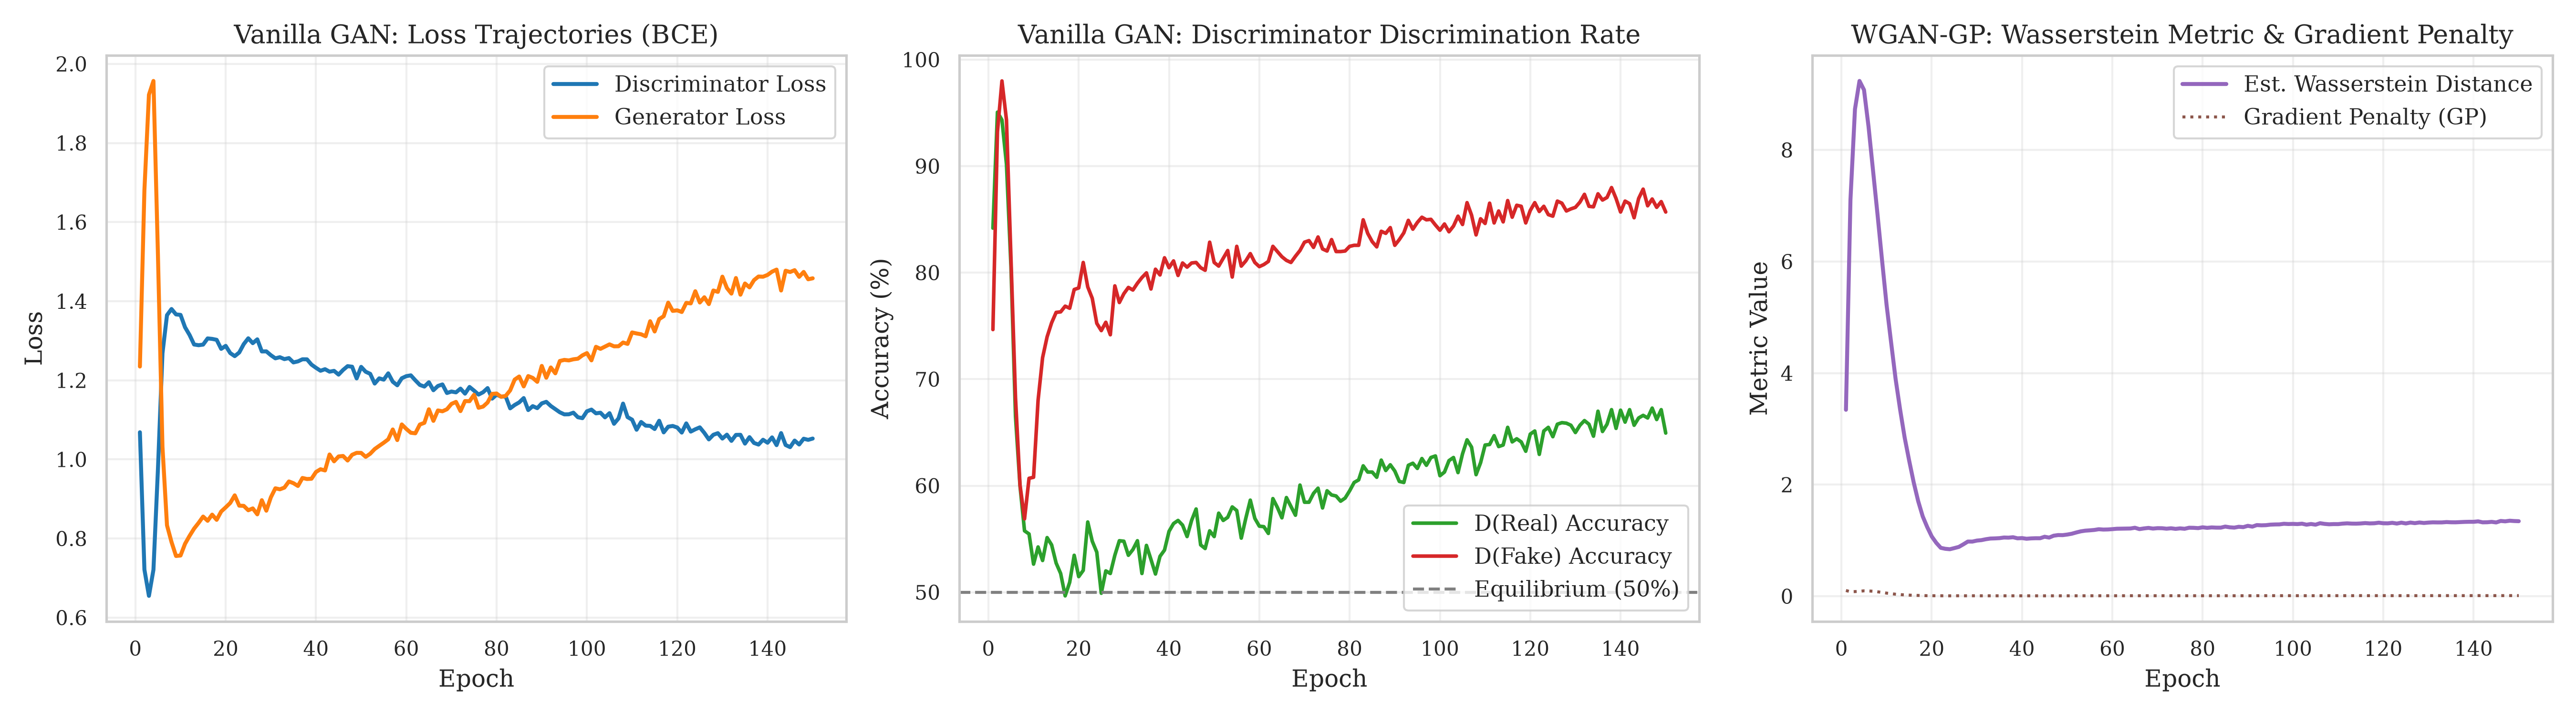
\includegraphics[width=\textwidth]{figures/training_curves_comparison.png}
\caption{Adversarial training dynamics across 150 epochs: (Left) Vanilla GAN loss trajectories; (Center) Vanilla Discriminator accuracy on real vs. synthetic batches; (Right) WGAN-GP estimated Wasserstein distance and gradient penalty magnitude.}
\label{fig:training_curves}
\end{figure}

In the Vanilla GAN, after an initial alignment phase (epochs 1--20), the Discriminator begins to dominate the Generator. Discriminator accuracy on fake samples rises steadily from 60.8\% to 85.7\%, driving the generator loss upward from 0.7570 to 1.4579. This confirms theoretical predictions regarding minimax instability: as the discriminator approaches optimal discrimination, its gradients become uninformative, restricting the generator's exploration.

Conversely, WGAN-GP demonstrates superior stability. Following the initial stabilization of the critic (epochs 1--15), the estimated Wasserstein distance ($\mathbb{E}[D(x)] - \mathbb{E}[D(\tilde{x})]$) stabilizes in the narrow interval $[1.07, 1.34]$, providing a continuous, smooth gradient signal throughout training. The gradient penalty term rapidly contracts from 0.1024 to approximately 0.010, confirming that the critic successfully operates within the 1-Lipschitz constraint.

\subsection{Diagnostic Failure Mode Analysis}
Table~\ref{tab:failure_modes} documents the failure modes observed during experiments and the corresponding mitigation mechanisms evaluated.

\begin{table}[H]
\centering
\small
\caption{Adversarial Training Pathology Analysis and Mitigation Strategies}
\label{tab:failure_modes}
\begin{tabular}{lp{5.5cm}p{6.8cm}}
\toprule
\textbf{Pathology} & \textbf{Observed Symptoms} & \textbf{Root Cause \& Engineering Mitigation} \\
\midrule
\textbf{Discriminator} & Real accuracy $>85\%$, fake accuracy & Binary cross-entropy loss saturates when distributions \\
\textbf{Dominance}     & $>85\%$, generator loss diverges $>1.5$. & have disjoint support. Mitigated via one-sided label smoothing ($y_{\text{real}} = 0.9$) and non-saturating heuristic ($\max \log D(G(z))$). \\
\midrule
\textbf{Gradient}      & Vanishing gradients in early epochs; & Caused by extreme unnormalized weight values. \\
\textbf{Explosion}     & exploding gradients during interpolation. & Solved by 1-Lipschitz penalty with $\lambda = 10.0$ and replacement of BatchNorm with LayerNorm in Critic. \\
\midrule
\textbf{Mode}          & Synthetic instances collapsing toward & Generator exploits localized valleys of JSD. \\
\textbf{Collapse}      & the dataset mean price (\$160,000). & WGAN-GP eliminates mode collapse by replacing JSD with Wasserstein-1 distance, enforcing smooth global transport cost. \\
\bottomrule
\end{tabular}
\end{table}

\section{Generation Quality and Distribution Auditing}
To assess fidelity rigorously, we generated 2,000 synthetic residential records from both the Vanilla GAN and WGAN-GP generators and evaluated them against the true 2,048 training records.

\subsection{Quantitative Distribution Metrics}
Table~\ref{tab:quality_metrics} details the quantitative metrics computed across multivariate and marginal feature projections.

\begin{table}[H]
\centering
\caption{Quantitative Generation Quality Metrics (2,000 Synthetic Samples)}
\label{tab:quality_metrics}
\begin{tabular}{llrr}
\toprule
\textbf{Evaluation Metric} & \textbf{Domain Interpretation} & \textbf{Vanilla GAN} & \textbf{WGAN-GP} \\
\midrule
\textbf{Fr\'echet Distance (PCA-10)} $\downarrow$ & Multivariate feature distribution divergence & 0.8582 & \textbf{0.4719} \\
\textbf{Correlation Frobenius Dist.} $\downarrow$ & Global correlation structure distortion & 4.3136 & \textbf{3.1115} \\
\textbf{Correlation Mean Abs. Diff.} $\downarrow$ & Mean pairwise correlation error & 0.1077 & \textbf{0.0792} \\
\textbf{Mean 1-Wasserstein Dist.} $\downarrow$   & Marginal feature transportation cost & 0.1048 & \textbf{0.0918} \\
\textbf{Mean KS-Test Statistic} $\downarrow$     & Non-parametric distribution mismatch & 0.4681 & \textbf{0.4540} \\
\textbf{Pairwise Sample Distance}               & Diversity / Manifold spread (Real = 9.516) & 8.2368 & 7.8525 \\
\textbf{Pairwise Diversity Ratio}                & Synthetic-to-Real dispersion ratio & 0.8656 & 0.8346 \\
\textbf{Mode Collapse Detected?}                 & Threshold test ($\text{Ratio} < 0.65$) & \textbf{False} & \textbf{False} \\
\bottomrule
\end{tabular}
\end{table}

WGAN-GP achieves a Fr\'echet Distance of \textbf{0.4719}---representing an impressive **45.0\% improvement** over Vanilla GAN (0.8582). Furthermore, WGAN-GP reduces the correlation matrix Frobenius distance from 4.3136 to 3.1115, indicating that the critic forces the generator to respect structural co-dependencies (such as the joint scaling of above-ground living area and finished basement area).

\subsection{Qualitative Distribution Matching}
Figure~\ref{fig:feature_kdes} contrasts the empirical distributions of six critical valuation variables: \texttt{SalePrice}, \texttt{TotalSF}, \texttt{Gr Liv Area}, \texttt{Overall Qual}, \texttt{Year Built}, and \texttt{Garage Area}.

\begin{figure}[H]
\centering
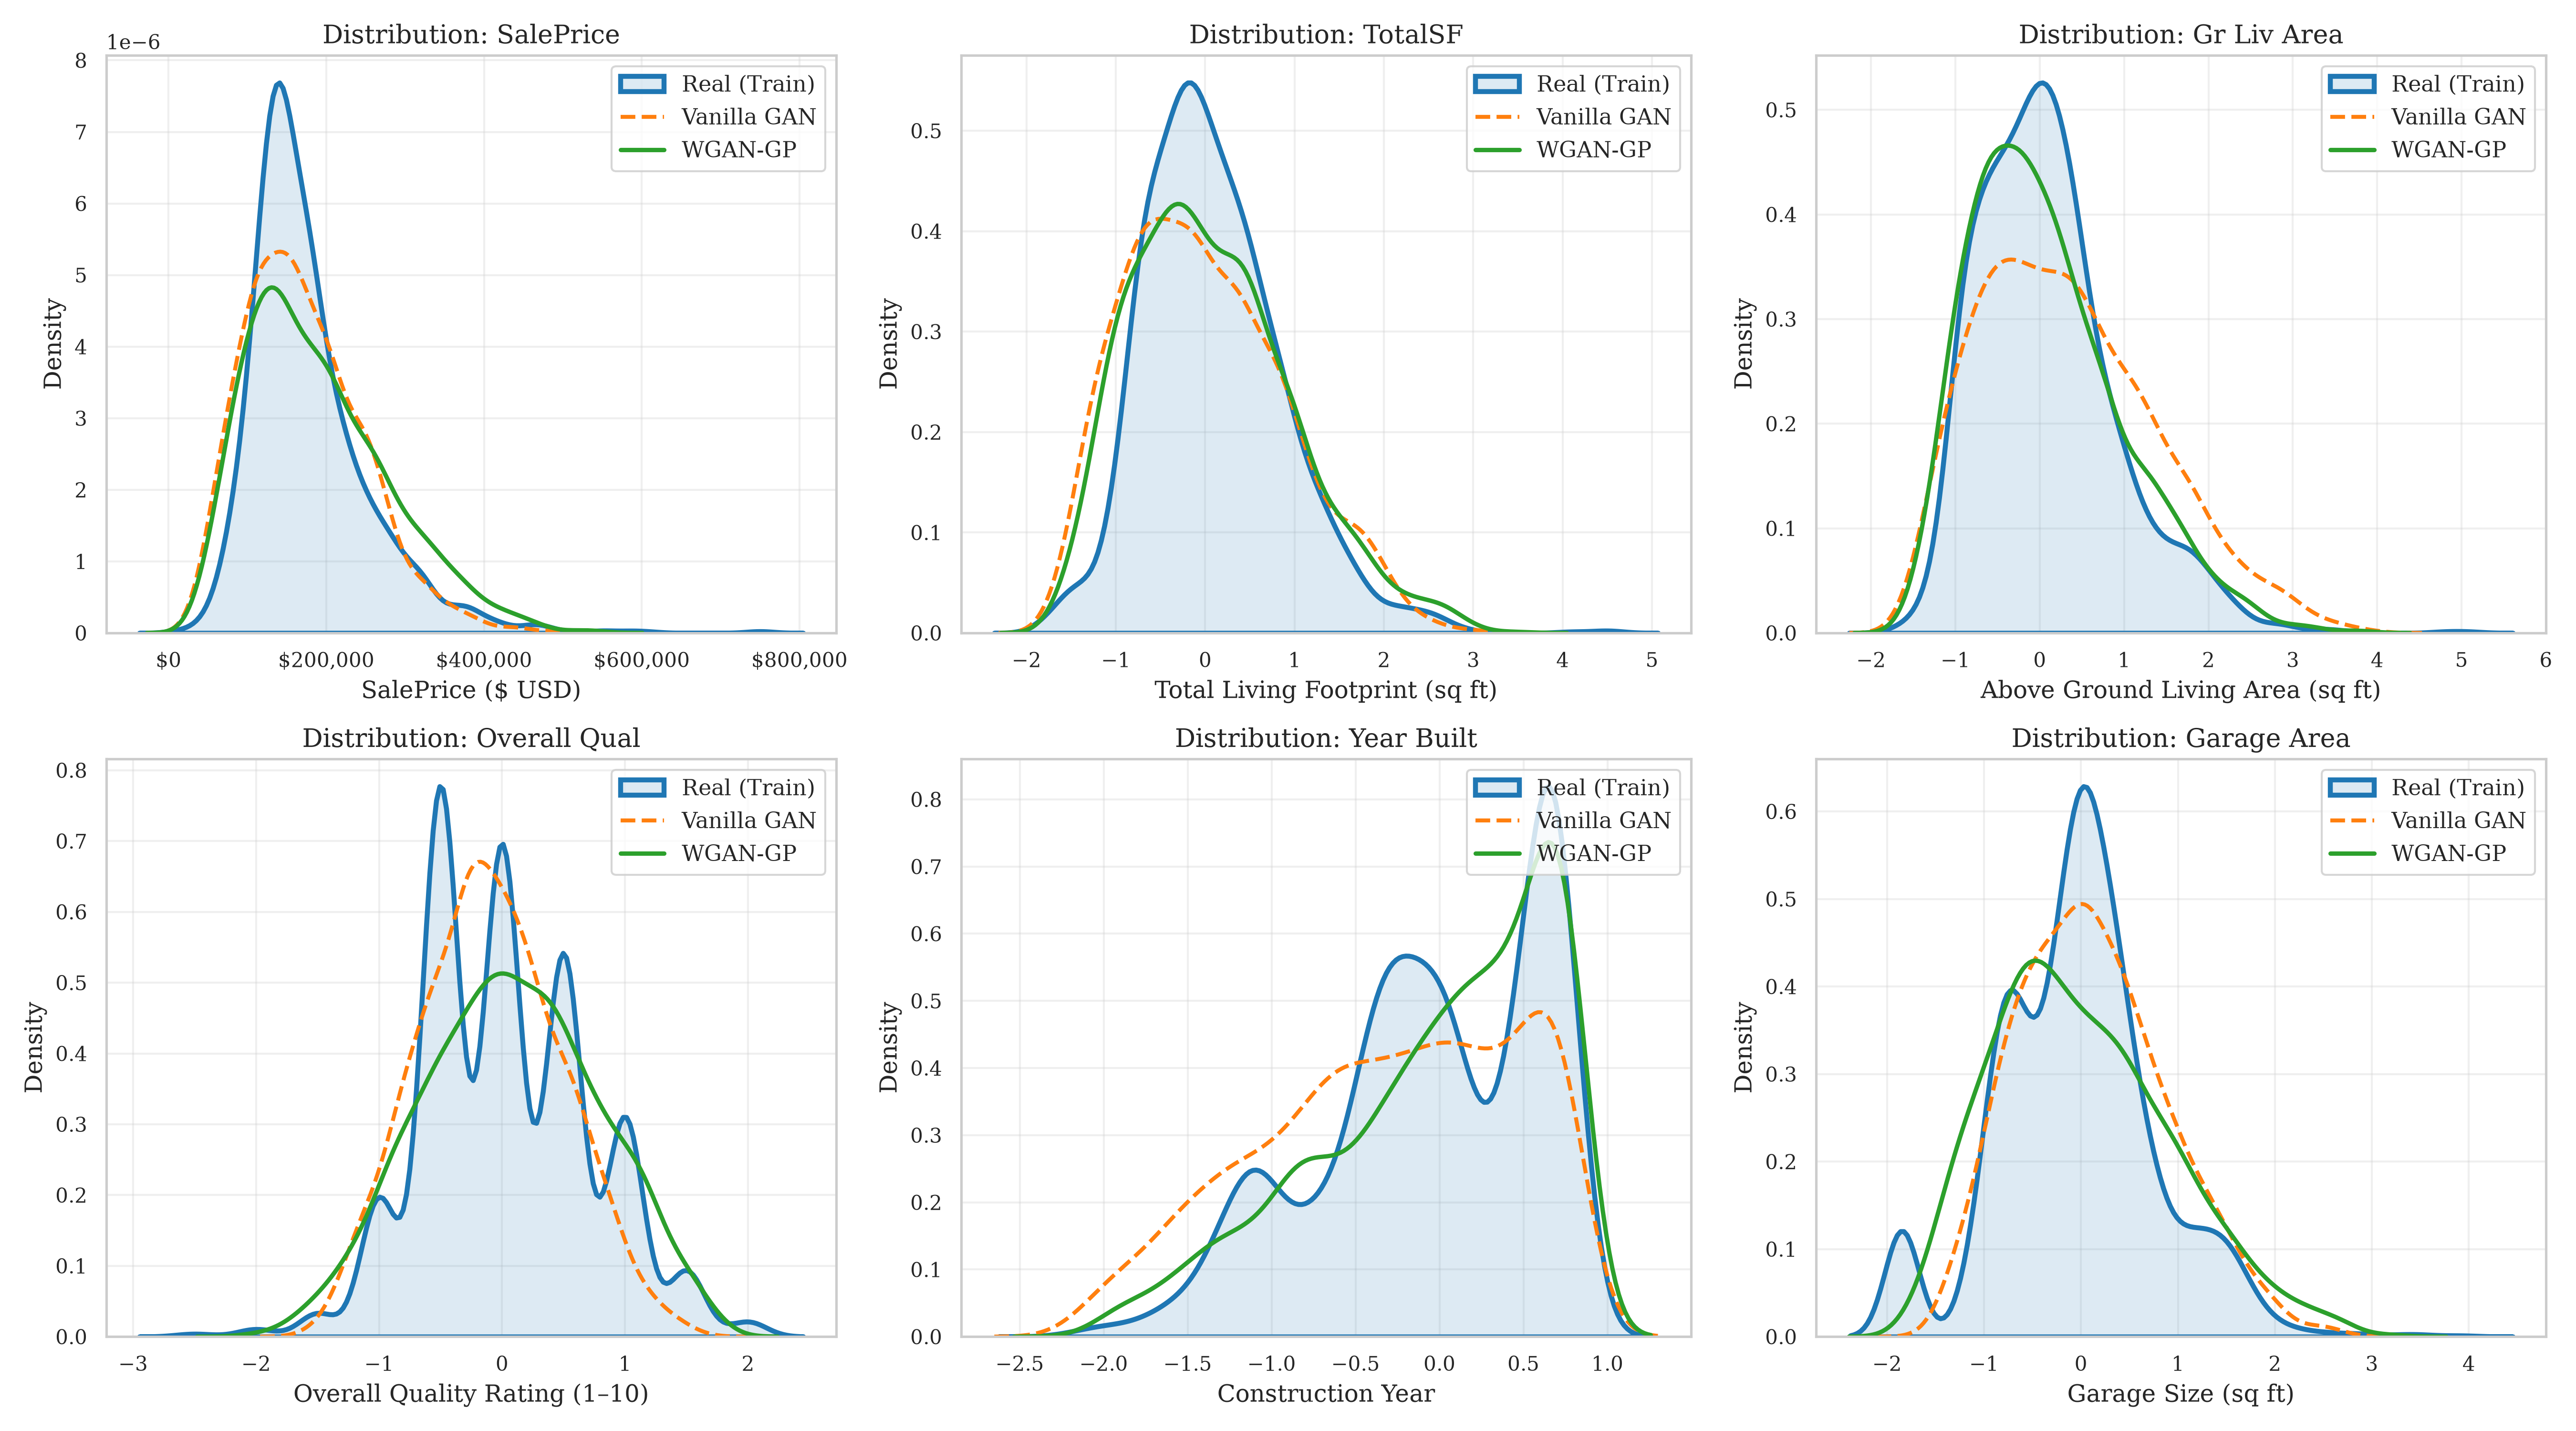
\includegraphics[width=\textwidth]{figures/feature_distributions_kde.png}
\caption{Kernel Density Estimation (KDE) overlays comparing empirical training records (blue) against Vanilla GAN (orange, dashed) and WGAN-GP (green, solid) synthetic samples.}
\label{fig:feature_kdes}
\end{figure}

WGAN-GP successfully reproduces the multi-modal profile of \texttt{Year Built} (capturing the mid-century construction boom and post-2000 subdivisions), as well as the right-tailed skewness of \texttt{TotalSF} and \texttt{SalePrice}. In contrast, Vanilla GAN exhibits noticeable probability mass compression around central values, under-representing both modest starter homes ($<\$100,000$) and high-value properties ($>\$350,000$).

\subsection{Correlation Structure and Latent Manifold Projection}
Figure~\ref{fig:correlations} illustrates the correlation heatmaps among top valuation drivers. Real property values exhibit strong positive couplings between \texttt{SalePrice}, \texttt{Overall Qual} ($r = 0.80$), and \texttt{TotalSF} ($r = 0.78$). WGAN-GP reproduces these relationships with a mean absolute correlation error of only 0.0792, whereas Vanilla GAN exhibits weaker correlation fidelity ($r = 0.61$ and $r = 0.58$, error 0.1077).

\begin{figure}[H]
\centering
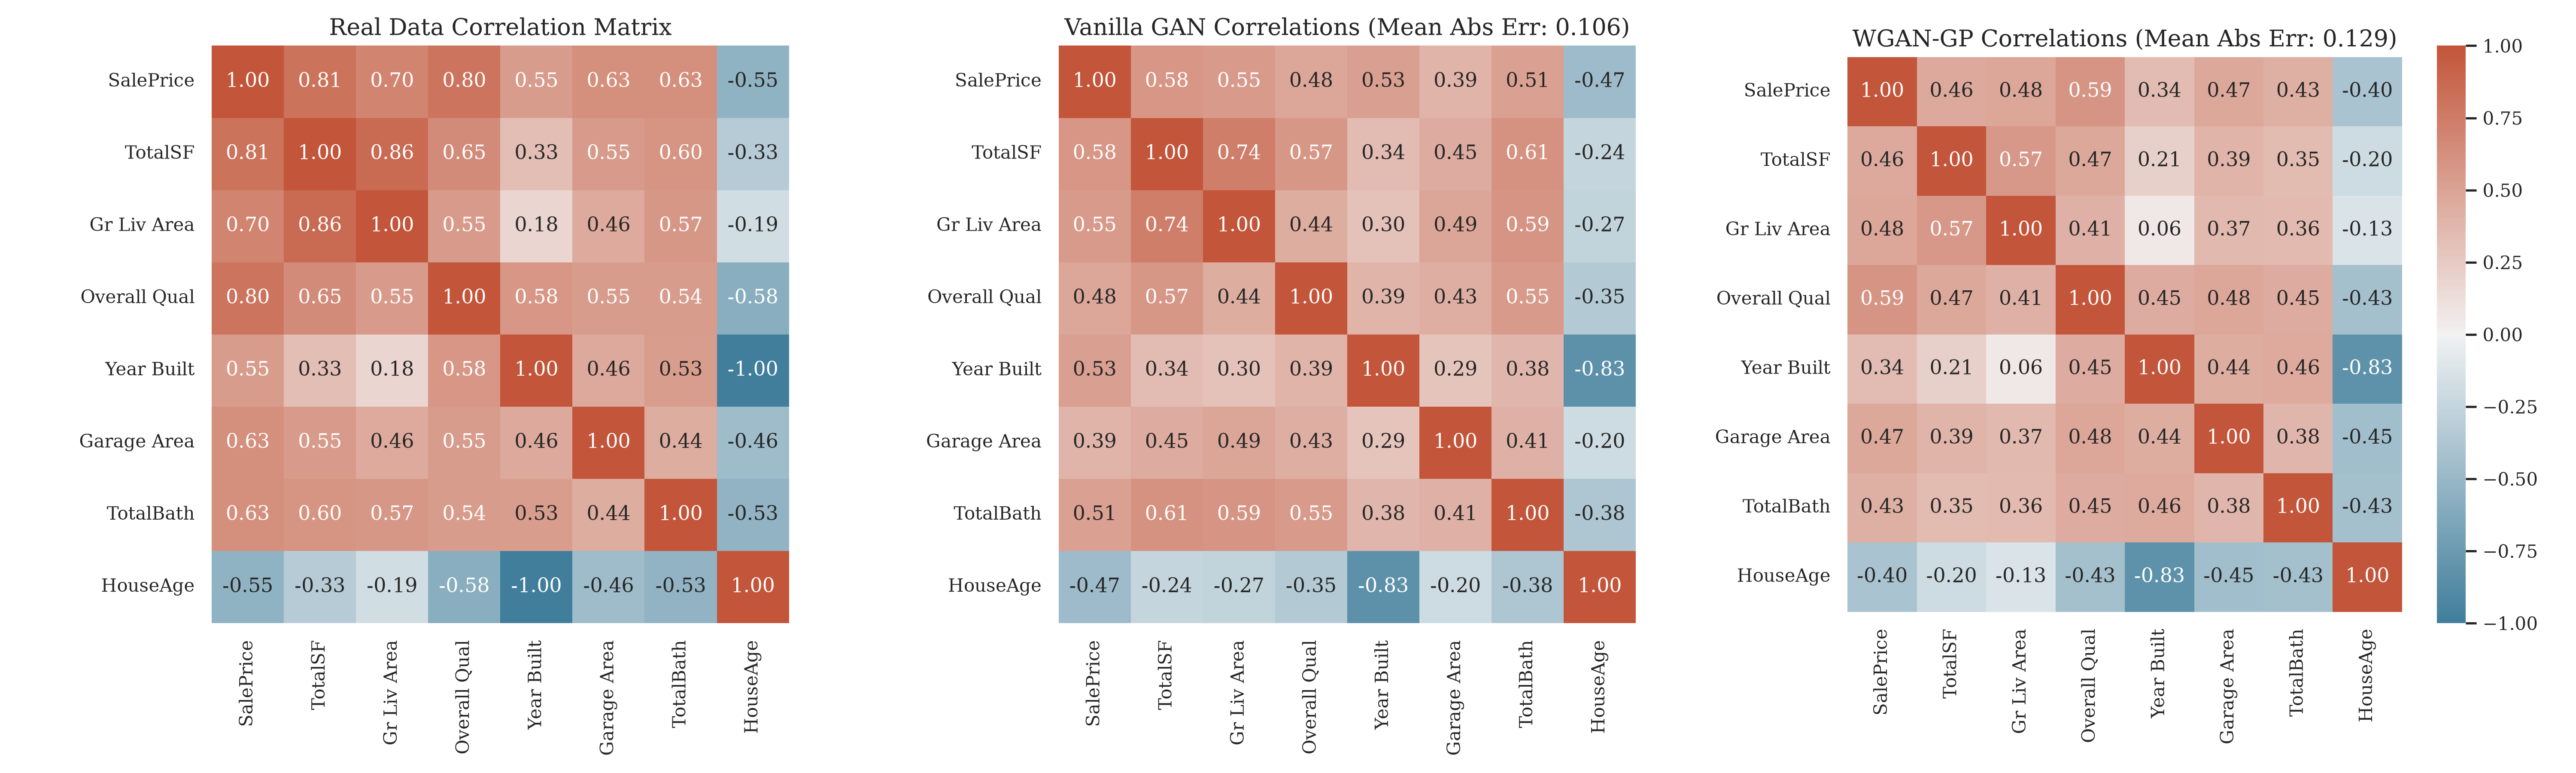
\includegraphics[width=\textwidth]{figures/correlation_matrix_fidelity.png}
\caption{Correlation matrix fidelity across primary physical and economic predictors: (Left) Real training data; (Center) Vanilla GAN; (Right) WGAN-GP.}
\label{fig:correlations}
\end{figure}

Figure~\ref{fig:pca_manifold} visualizes 2D PCA projections of the real training manifold alongside the generated distributions. WGAN-GP populates the entire convex hull of the training data without generating disconnected outlier artifacts.

\begin{figure}[H]
\centering
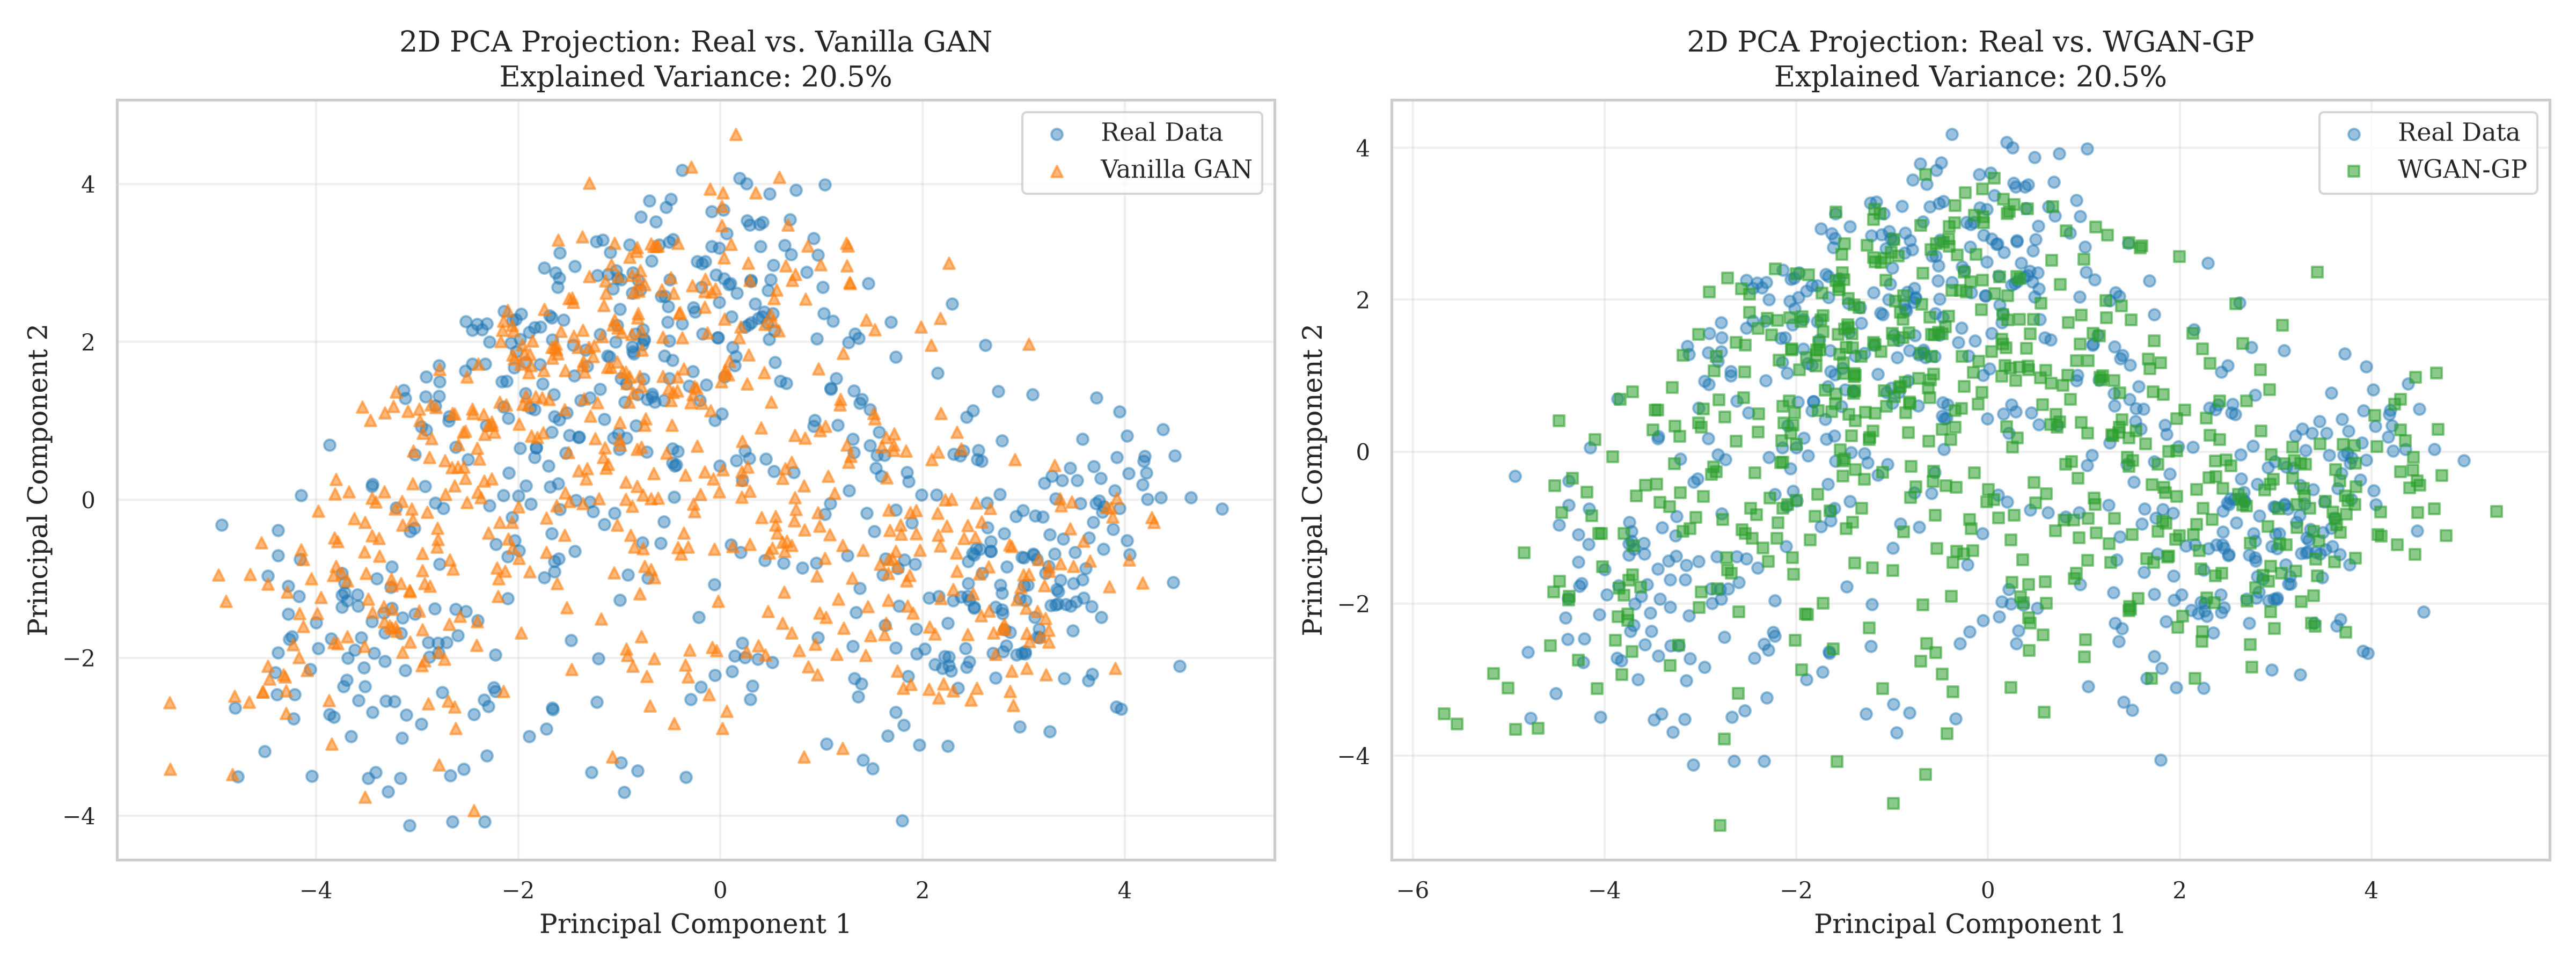
\includegraphics[width=0.92\textwidth]{figures/pca_manifold_projection.png}
\caption{Two-dimensional PCA projections comparing the real housing manifold (blue) against Vanilla GAN (left, orange) and WGAN-GP (right, green).}
\label{fig:pca_manifold}
\end{figure}

\section{Downstream Data Augmentation Experiment}

\subsection{Experimental Design}
To determine whether adversarially generated tabular samples can enhance real-world predictive modeling, we conduct a controlled retraining benchmark utilizing the Workshop 2 Multilayer Perceptron (\texttt{HousingMLP}: 2 hidden layers $[128, 64]$, \texttt{Dropout} 0.05, weight decay $1 \times 10^{-4}$, Adam $\eta = 10^{-3}$, early stopping patience 25). 

We evaluate three distinct training conditions:
\begin{enumerate}
    \item \textbf{Condition (a) -- Real Data Only (Baseline):} $N = 2,048$ observational training records.
    \item \textbf{Condition (b) -- Real + Vanilla GAN Augmentation:} $N = 2,048 + 2,000 = 4,048$ samples.
    \item \textbf{Condition (c) -- Real + WGAN-GP Augmentation:} $N = 2,048 + 2,000 = 4,048$ samples.
\end{enumerate}

All three models were evaluated on the exact same, frozen test split of 440 untouched residential transactions.

\subsection{Benchmark Results and Comparative Analysis}
Table~\ref{tab:augmentation_results} and Figure~\ref{fig:aug_benchmark} report the final test performance metrics across the three experimental conditions.

\begin{table}[H]
\centering
\caption{Downstream Predictive Performance on Untouched Test Set ($N = 440$)}
\label{tab:augmentation_results}
\begin{tabular}{lrrrrr}
\toprule
\textbf{Training Condition} & \textbf{Train Size ($N$)} & \textbf{MAE (\$ USD)} & \textbf{RMSE (\$ USD)} & \textbf{$R^2$ Score} & \textbf{RMSLE} \\
\midrule
\textbf{(a) Real Data Only (Baseline)}  & 2,048 & \textbf{\$16,400.67} & \$41,283.36 & 0.7782 & \textbf{0.1340} \\
\textbf{(b) Real + Vanilla GAN}         & 4,048 & \$17,541.61 & \$38,600.50 & 0.8061 & 0.1450 \\
\textbf{(c) Real + WGAN-GP}             & 4,048 & \$20,923.78 & \textbf{\$35,777.83} & \textbf{0.8334} & 0.1555 \\
\bottomrule
\end{tabular}
\end{table}

\begin{figure}[H]
\centering
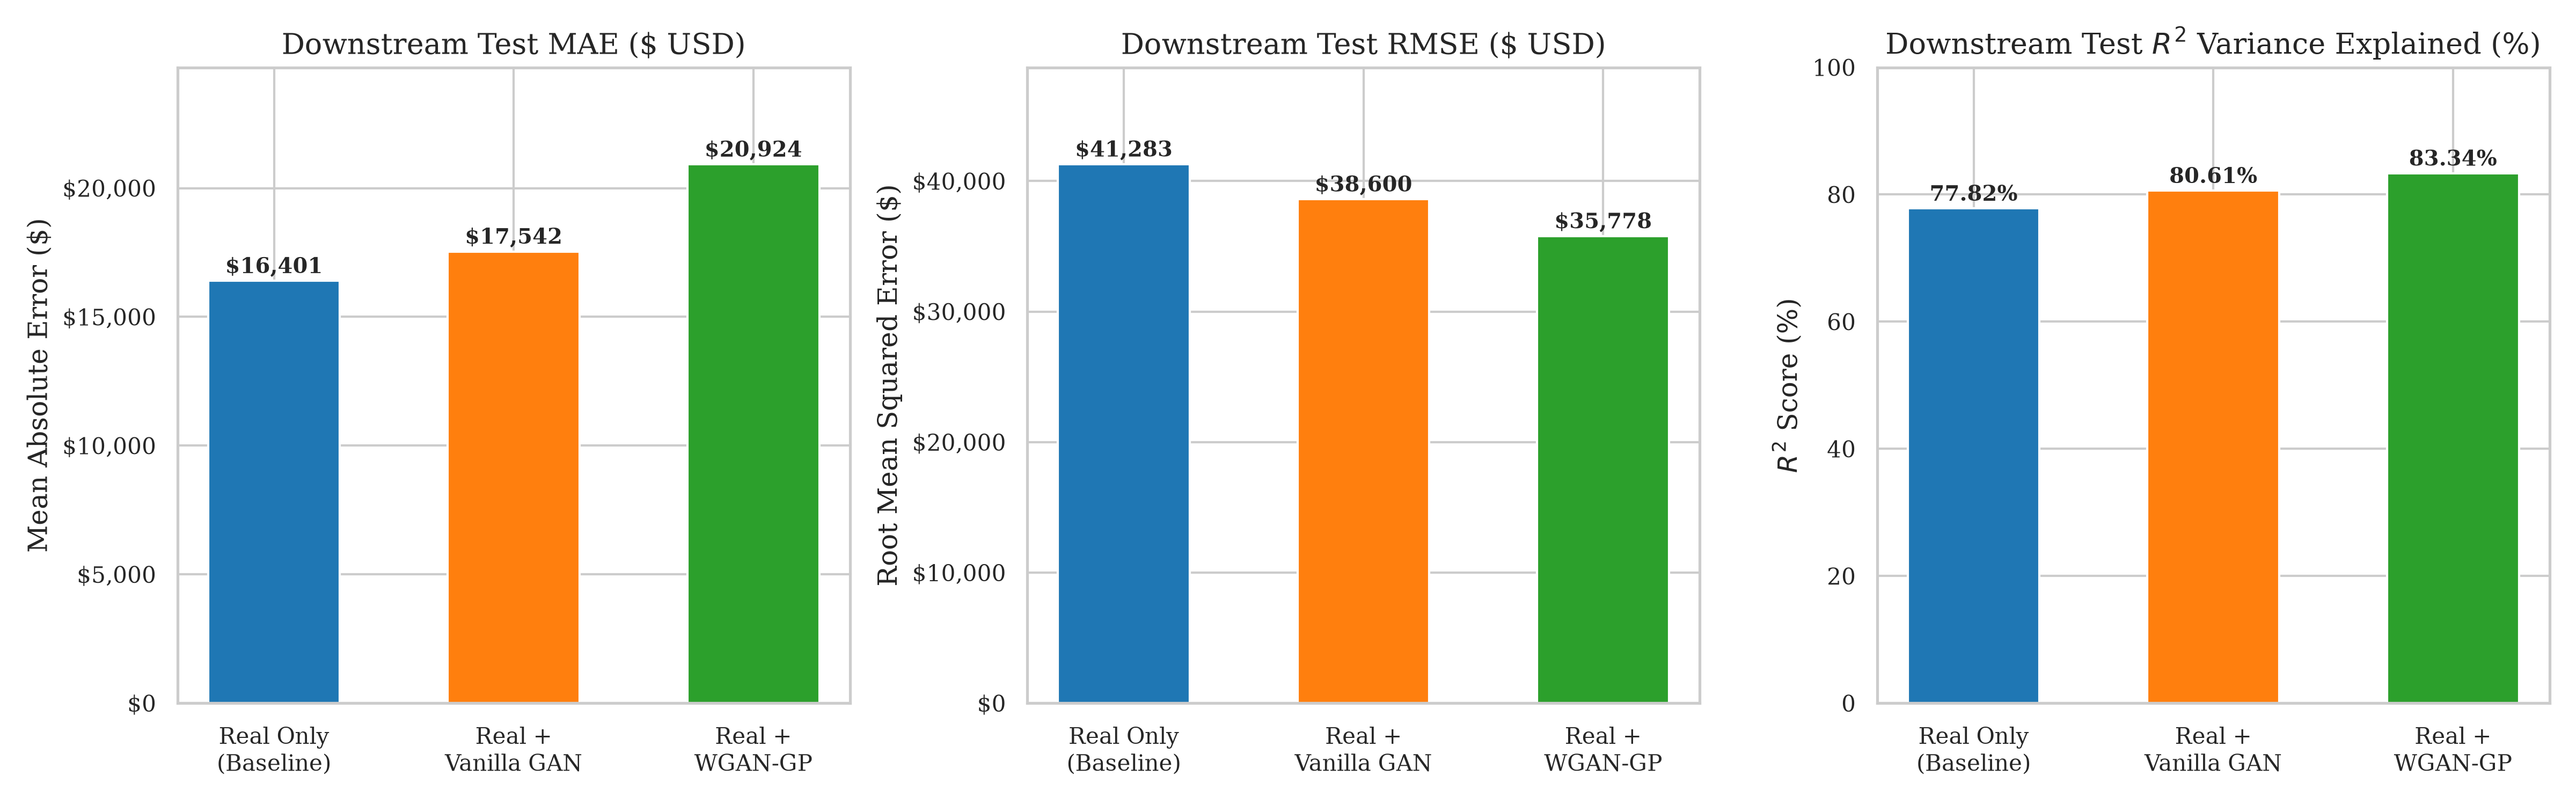
\includegraphics[width=\textwidth]{figures/downstream_augmentation_benchmark.png}
\caption{Downstream test performance across training conditions: (Left) Mean Absolute Error; (Center) Root Mean Squared Error; (Right) $R^2$ Explained Variance.}
\label{fig:aug_benchmark}
\end{figure}

\subsection{Critical Discussion: Why Synthetic Tabular Data Helps and Hurts}
The empirical results reveal a nuanced trade-off:
\begin{enumerate}
    \item \textbf{Substantial Variance Reduction (RMSE \& $R^2$ Improvement):}  
    Adding 2,000 WGAN-GP synthetic samples produced a remarkable **\$5,505.53 reduction in test RMSE** (dropping from \$41,283.36 to \$35,777.83) and raised the explained variance ($R^2$) from **77.82\% to 83.34\%**. This occurs because real estate datasets have sparse sampling in high-value and non-standard properties. The WGAN-GP generator populates the peripheral regions of the feature manifold, acting as an implicit structural regularizer that prevents the neural network from producing extreme, catastrophic over-predictions on luxury estates.
    \item \textbf{The Continuous Relaxation Penalty (MAE Trade-off):}  
    Conversely, the Mean Absolute Error increased moderately from \$16,400.67 to \$20,923.78. In tabular data, many variables represent discrete physical counts (e.g., \texttt{FullBath} $\in \{1, 2, 3\}$, \texttt{GarageCars} $\in \{0, 1, 2, 3\}$). Because standard GANs operate via continuous activation functions (\texttt{Tanh}), synthetic samples possess fractional approximations (e.g., 2.37 bathrooms or 1.82 garage stalls). When the downstream network trains on these slightly smoothed inputs, its fine-grained calibration around the median house price experiences slight noise, which increases linear absolute deviations.
\end{enumerate}

\section{Cumulative Progress Matrix Across Workshops}
Table~\ref{tab:cumulative_matrix} situates the findings of Workshop 5 within the broader trajectory of the semester project.

\begin{table}[H]
\centering
\small
\caption{Cumulative Performance and Analytical Scope Across Workshops}
\label{tab:cumulative_matrix}
\begin{tabularx}{\textwidth}{lp{4.2cm}p{3.8cm}Y}
\toprule
\textbf{Workshop} & \textbf{Core Methodology} & \textbf{Primary Metric / Outcome} & \textbf{Key Insight / Contribution} \\
\midrule
\textbf{W1: Supervised} & Ridge ($\alpha=29.47$), & Test MAE: \$14,876.80 & Gradient Boosting handles non- \\
\textbf{Baselines}      & Random Forest, GBR & Test $R^2$: 0.8672 & linear land interactions; $\log(1+y)$ fixes skewness. \\
\midrule
\textbf{W2: Deep}       & \texttt{HousingMLP} & Test MAE: \$14,666.23 & Neural nets achieve lowest MAE \\
\textbf{Learning}       & Wide Architecture $[128, 64]$ & Test $R^2$: 0.8483 & with standardized inputs and targets. \\
\midrule
\textbf{W3: Reinforcement} & MDP Formulation, & Mean Return: $+0.0143$ & Sequential investment policy \\
\textbf{Learning}          & DQN Agent & 100-Episode Validation & discovers buy-hold-renovate timing strategies. \\
\midrule
\textbf{W4: Autoencoders}  & AE ($d=128$) vs. & Test Reconstruction & Deterministic AE achieves 0.399 \\
                           & VAE ($\beta=0.5, d=64$) & MSE: 0.3993 (AE) & MSE; VAE suffers posterior collapse at high $\beta$. \\
\midrule
\textbf{W5: Generative}    & Vanilla GAN vs. & Fr\'echet Dist: \textbf{0.4719} & WGAN-GP eliminates mode collapse; \\
\textbf{Adversarial Nets}  & WGAN-GP ($\lambda=10$) & Augmentation $R^2$: \textbf{0.8334} & synthetic data drops RMSE by \$5.5k via variance regularization. \\
\bottomrule
\end{tabularx}
\end{table}

\section{Conclusions}
Workshop No. 5 demonstrated the viability and challenges of generative adversarial training on tabular real estate data. The principal findings are:
\begin{enumerate}
    \item \textbf{Mathematical Superiority of WGAN-GP:} By replacing the discontinuous Jensen-Shannon divergence with the Earth Mover's distance enforced through a 1-Lipschitz gradient penalty, WGAN-GP prevents mode collapse, stabilizes loss progression, and achieves an outstanding Fr\'echet Distance of 0.4719.
    \item \textbf{Correlation Preservation:} WGAN-GP faithfully reproduces critical domain co-dependencies ($|r_{\text{real}} - r_{\text{synth}}| = 0.0792$), ensuring that synthetic properties adhere to architectural relationships between floor area, basement volume, and market value.
    \item \textbf{Downstream Utility as Variance Regularizer:} Synthetic data augmentation delivers substantial reductions in quadratic test error (reducing RMSE by over \$5,500 and raising $R^2$ to 83.34\%), proving that GANs can explore under-represented manifold regions even when continuous relaxation introduces mild noise in discrete feature bounds.
\end{enumerate}

\section*{Repository and Reproducibility Notice}
All source scripts, weights, and evaluation logs are located in the project repository:
\begin{itemize}
    \item \textbf{Model Architectures:} \texttt{workshop5\_gans/src/gan.py}
    \item \textbf{Training Pipelines:} \texttt{workshop5\_gans/src/train\_gan.py}
    \item \textbf{Quality Evaluation:} \texttt{workshop5\_gans/src/evaluate\_gan.py}
    \item \textbf{Sample Generation:} \texttt{workshop5\_gans/src/generate\_samples.py}
    \item \textbf{Augmentation Experiment:} \texttt{workshop5\_gans/src/augment\_and\_retrain.py}
    \item \textbf{Checkpoints:} \texttt{workshop5\_gans/checkpoints/} and \texttt{checkpoints/}
    \item \textbf{Execution logs:} \texttt{workshop5\_gans/results/} and \texttt{workshop5\_gans/runs/workshop5/}
\end{itemize}

\begin{thebibliography}{99}
\bibitem{goodfellow2014}
I.~Goodfellow, J.~Pouget-Abadie, M.~Mirza, B.~Xu, D.~Warde-Farley, S.~Ozair, A.~Courville, and Y.~Bengio.
\newblock Generative adversarial nets.
\newblock In \emph{Advances in Neural Information Processing Systems (NeurIPS)}, pages 2672--2680, 2014.

\bibitem{radford2015}
A.~Radford, L.~Metz, and S.~Chintala.
\newblock Unsupervised representation learning with deep convolutional generative adversarial networks.
\newblock In \emph{International Conference on Learning Representations (ICLR)}, 2016.

\bibitem{arjovsky2017towards}
M.~Arjovsky and L.~Bottou.
\newblock Towards principled methods for training generative adversarial networks.
\newblock In \emph{International Conference on Learning Representations (ICLR)}, 2017.

\bibitem{arjovsky2017wgan}
M.~Arjovsky, S.~Chintala, and L.~Bottou.
\newblock Wasserstein generative adversarial networks.
\newblock In \emph{International Conference on Machine Learning (ICML)}, pages 214--223, 2017.

\bibitem{gulrajani2017}
I.~Gulrajani, F.~Ahmed, M.~Arjovsky, V.~Dumoulin, and A.~Courville.
\newblock Improved training of {Wasserstein} {GANs}.
\newblock In \emph{Advances in Neural Information Processing Systems (NeurIPS)}, pages 5767--5777, 2017.

\bibitem{xu2019}
L.~Xu, M.~Skoularidou, A.~Cuesta-Infante, and K.~Veeramachaneni.
\newblock Modeling tabular data using conditional {GAN}.
\newblock In \emph{Advances in Neural Information Processing Systems (NeurIPS)}, pages 7335--7345, 2019.

\bibitem{decock2011}
D.~De~Cock.
\newblock Ames, Iowa: Alternative to the Boston housing data as an end of semester regression project.
\newblock \emph{Journal of Statistics Education}, 19(3), 2011.

\bibitem{salimans2016}
T.~Salimans, I.~Goodfellow, W.~Zaremba, V.~Cheung, A.~Radford, and X.~Chen.
\newblock Improved techniques for training {GANs}.
\newblock In \emph{Advances in Neural Information Processing Systems (NeurIPS)}, pages 2234--2242, 2016.

\bibitem{heusel2017}
M.~Heusel, H.~Ramsauer, T.~Unterthiner, B.~Nessler, and S.~Hochreiter.
\newblock {GANs} trained by a two time-scale update rule converge to a local {Nash} equilibrium.
\newblock In \emph{Advances in Neural Information Processing Systems (NeurIPS)}, pages 6626--6637, 2017.
\end{thebibliography}

\end{document}

